\documentclass[]{beamer}
% Class options include: notes, notesonly, handout, trans,
%                        hidesubsections, shadesubsections,
%                        inrow, blue, red, grey, brown

% Theme for beamer presentation.
\usepackage{beamerthemesplit} 
\usepackage[utf8]{inputenc}
\usepackage[T1]{fontenc}
\usepackage[english,swedish]{babel}
% Other themes include: beamerthemebars, beamerthemelined, 
%                       beamerthemetree, beamerthemetreebars  

\graphicspath{{figures/}{figures/hmm-graph/}{figures/gwhisker_database/}{figures/gwhiskers/}}

\title{Probabilistic Tracking of Multiple Whiskers}
\author{Jim Holmstr\"{o}m, Emil Lundberg}                 % Enter your name between curly braces
\institute{CSC,KTH}      % Enter your institute name between curly braces
\date{\today}                    % Enter the date or \today between curly braces

\renewcommand{\ae}{\"{a}}
\renewcommand{\oe}{\"{o}}
\renewcommand{\AE}{\"{A}}
\renewcommand{\OE}{\"{O}}

\newcommand{\prob}[1]{p\left(#1\right)}
\newcommand{\cprob}[2]{\prob{\left. #1 \middle\vert #2 \right.}}
\newcommand{\cprobnext}[1]{\cprob{#1_{n+1}}{#1_n}}
\newcommand{\ndist}[2]{\mathcal{N}\left(#1, #2\right)}
\newcommand{\norm}[1]{\left\|#1\right\|}
\newcommand{\Lp}[1]{\mathrm{L}^{#1}}

\begin{document}

% Creates title page of slide show using above information
\begin{frame}
  \titlepage
\end{frame}
\note{Talk for 30 minutes} % Add notes to yourself that will be displayed when
                           % typeset with the notes or notesonly class options

% slides are 3in high by 5in wide

\section{Bakgrund}
\begin{frame}
  \frametitle{Bakgrund}
  \begin{columns}[c]
    \column{2in}
    \begin{itemize}
    \item Neurofysiologer vill studera rörelser hos morrh\aa r
    \item Befintliga kommersiella l\oe sningar \ae r dyra eller kr\ae ver inskr\ae nkningar
    \end{itemize}
    \column{2in}
    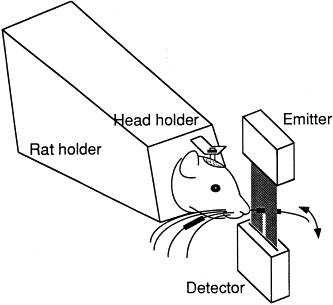
\includegraphics[width=0.75\textwidth]{optoelectronic.png}
  \end{columns}
\end{frame}

\section[Agenda]{}

% Creates table of contents slide incorporating
% all \section and \subsection commands
\begin{frame}
  \tableofcontents
\end{frame}

\section{Probabilistisk metod}

\subsection{Dold Markovmodell}
\begin{frame}
\frametitle{Dold Markovmodell}
  \begin{columns}[c]
    \column{2in}
    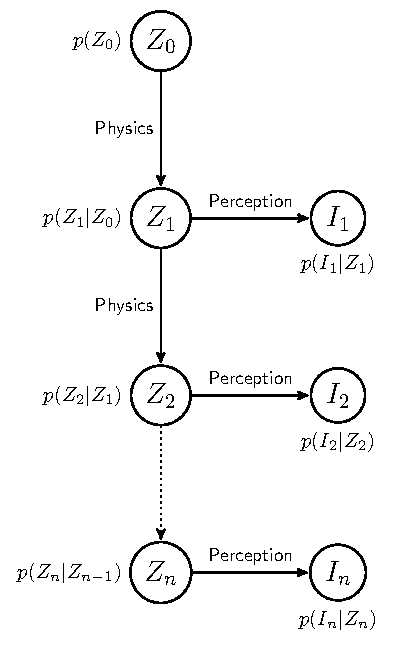
\includegraphics[width=0.8\textwidth]{hmm-graph.pdf}
    
    \column{2in}
    \begin{itemize}
    \item System \oe verg\aa r mellan tillst\aa nd med sannolikheter $\cprobnext{Z}$
    \item Tillst\aa ndet kan ej m\ae tas direkt
    \item F\aa r ist\ae llet en \emph{observation} $I_n$ av tillst\aa ndet $Z_n$ med sannolikhet $\cprob{I_n}{Z_n}$
    \end{itemize}
  \end{columns}
\end{frame}

\subsection{Partikelfiltret}

\begin{frame}
  \frametitle{Partikelfiltret}
  \begin{center}
    Approximerar sannolikhetsf\oe rdelning med diskreta m\ae ngder
    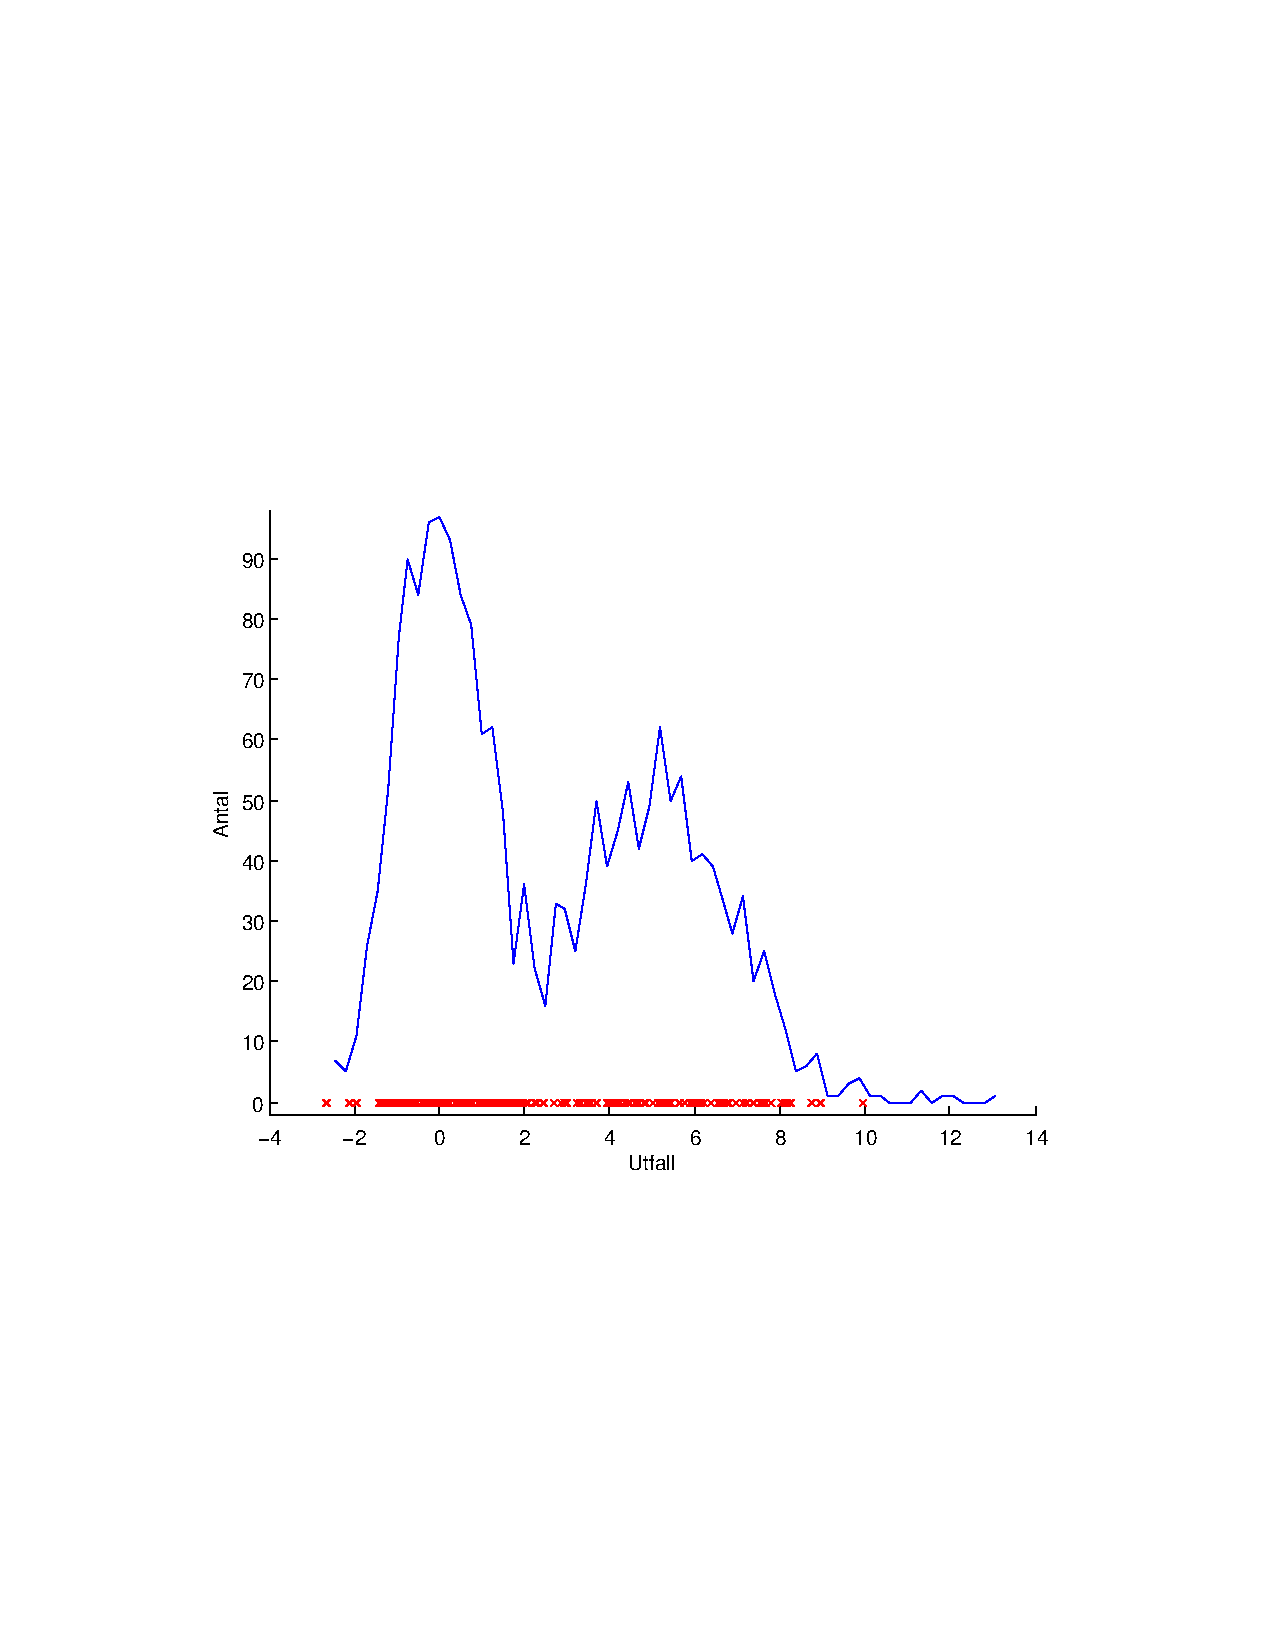
\includegraphics[trim=3cm 8cm 4cm 8cm, clip=true, totalheight=0.7\textheight]{hist.pdf}
  \end{center}
\end{frame}

\begin{frame}
  
  \begin{columns}[tt]
    \column{2.5in}
    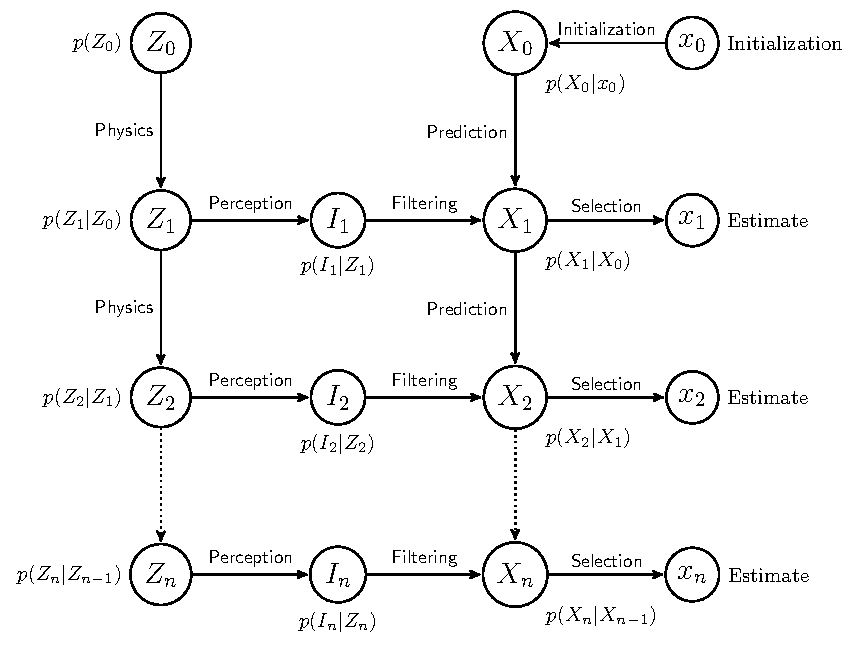
\includegraphics[width=1\textwidth]{hmm-graph-pf.pdf}

    \column{2.5in}
    \begin{itemize}
    \item Fyra steg:
    \end{itemize}
    \begin{description}
    \item[Prediktion] Skapa hypoteser om n\ae sta tidssteg
    \item[Perception] L\ae s in och tolka bild
    \item[Filtrering] V\ae lj ut de hypoteser f\oe r vilka bilden \ae r trolig
    \item[Urval] Konstruera en uppskattning av systemet utifr\aa n de filtrerade hypoteserna
    \end{description}
    
  \end{columns}
\end{frame}

\begin{frame}
  \begin{columns}[c]
    \column{2.5in}

    \begin{description}
      \item[\color{red}{
          \begin{picture}(0, 0)
            \color{blue}
            \put(-16, 4){\circle{16}}
          \end{picture}}] F\oe re filtrering
      \item[]
      \item[\color{red}{
          \begin{picture}(0, 0)
            \color{red}
            \put(-16, 4){\circle{16}}
          \end{picture}}] Efter filtrering
      \item[]
      \item[\color{red}{
          \begin{picture}(0, 0)
            \color{green}
            \put(-16, 4){\circle{16}}
          \end{picture}}] Slutlig uppskattning
    \end{description}
    
    \column{2in}
    
    \begin{center}
      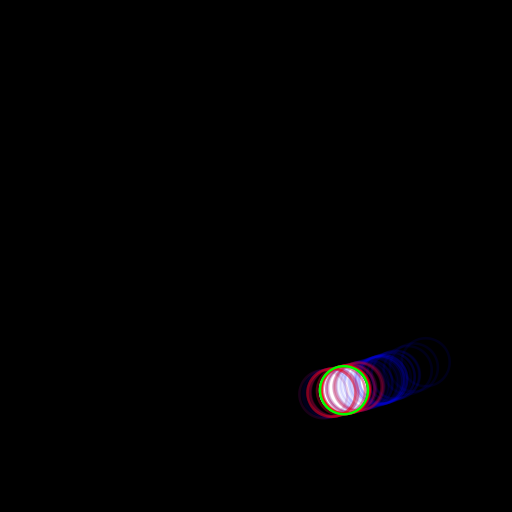
\includegraphics[width=1\textwidth]{pendulum-tracking.png}
    \end{center}
  \end{columns}
\end{frame}

\subsection{Morrh\aa rens Matematiska Modell}
\begin{frame}
  \frametitle{Morrh\aa rens Matematiska Modell}

  \begin{columns}[c]
    \column{3in}
    \begin{itemize}
    \item Mycket enkel modell: $a_1x + a_2x^2 + a_3x^3$
      \begin{itemize}
      \item Approximerar morrh\aa rens form inom felmarginal f\oe r blotta \oe gat
      \item Kan missa lite i s\ae llsynta extrema fall
      \end{itemize}
    \item Andra kandidater t.ex. $\sum\limits_k a_k\sin \left(kx\right)$
    \end{itemize}
    
    \column{1.5in}
    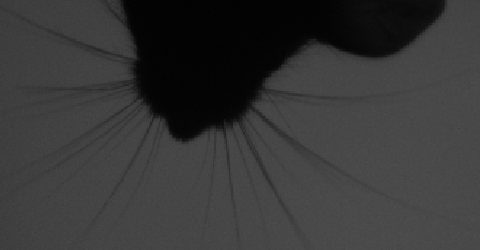
\includegraphics[width=1\textwidth]{rat-vanilla.png}

    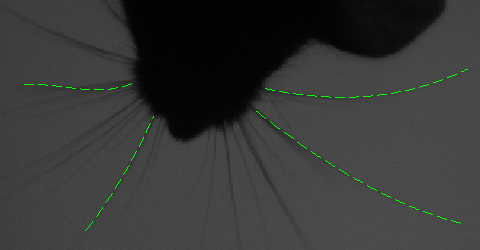
\includegraphics[width=1\textwidth]{rat-splines.png}
  \end{columns}
\end{frame}

\end{document}
